\chapter[Transfer Learning]{Transfer Learning}
\label{ch:transfer-learning}\index{transfer learning|(}

Machine learning algorithms typically operate within isolated problem domains - for example, a model trained to recognize motorcycles would not aim to recognize bicycles. However, this approach is not an accurate representation of human intelligence; in fact, we know that humans can relate knowledge of motorcycles to bicycles \citep{aytar2011}. 

Unlike classical machine learning approaches, human beings instinctively learn from different sources, drawing from varied past experiences and transferring knowledge across different contexts. 

Transfer Learning is the study of extending classical machine learning approaches to apply knowledge acquired from a number of source tasks, to a different but related target task, similar to the way humans learn \citep{thrunpratt1998}. 

\begin{marginfigure}
  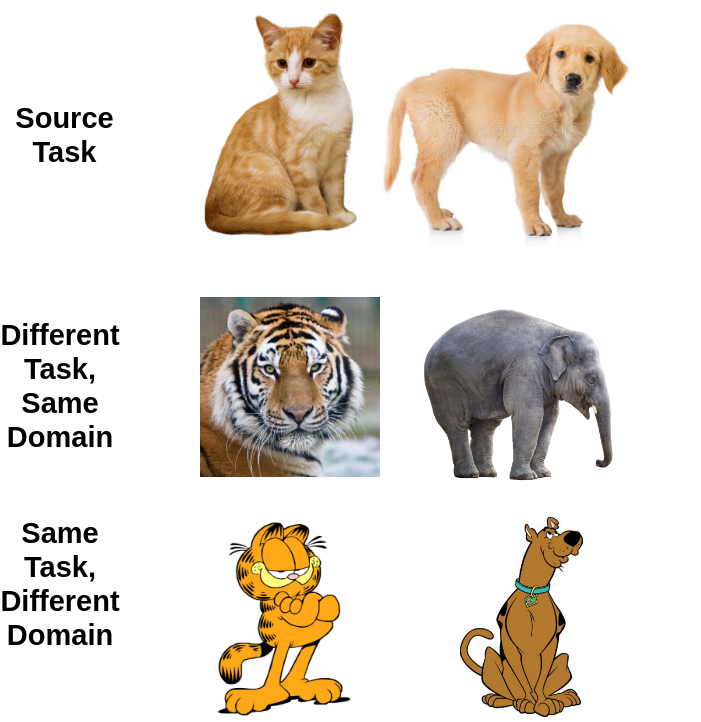
\includegraphics{transfer_learning/transfer-learning-domain-and-tasks.png}
  \caption{Transfer learning can occur across domains or across tasks. Images reproduced from commons.wikimedia.org (Tiger, Cartoon Cat), imdb.com (Cartoon Dog), pixabay.com (Cat), pnghunter.com (Elephant) and shutterstock.com (Dog).}
  \label{fig:transferlearning_domaintask}
\end{marginfigure}



Source tasks and target tasks can be related in different ways. For example, if a source task is a \textit{'Dog or Cat'} classifier; we can transfer knowledge to a similar domain but a different task, such as an \textit{'Elephant or Tiger'} classifier; or we can transfer knowledge to the same task in a different domain, such as a \textit{'Cartoon Dog or Cat'} classifier \citep{torrey2009}. 


\section{Transfer Learning Approaches}\label{sec:transfer-learning-approaches}\index{transfer learning!transfer learning approaches}

When labeled data is in short supply or learning is computationally expensive and time consuming, one may select a surrogate task to train for, and transfer knowledge to the intended target task.  This is especially beneficial in cases where we do not have enough data, or where training and test data do not possess the same characteristics; containing a different feature space, different distributions, different data sources or even different target labels. 

In fact, Transfer Learning approaches can be generalised into three categories, depending on the availability of labeled data for the source and target tasks \citep{panyang2010}:
\begin{enumerate}  
\item \textbf{Inductive Transfer Learning;} applicable when data is available for the target domain. Cases where there is no data for the source domain are referred to as self-taught learning; whereas cases where data is also available in the source domain is referred to as multi-task learning.




\item \textbf{Transductive Transfer Learning;} applicable when where labeled data is only available in the source domain. Transductive learning where we assume the same task but different domains is referred to as domain adaptation, while learning a similar domain but a different task is referred to as Sample Bias Selection.  

\item \textbf{Unsupervised Transfer Learning;} applicable when labelled data is not available neither for the source nor the target task.
\end{enumerate}

\begin{figure}
  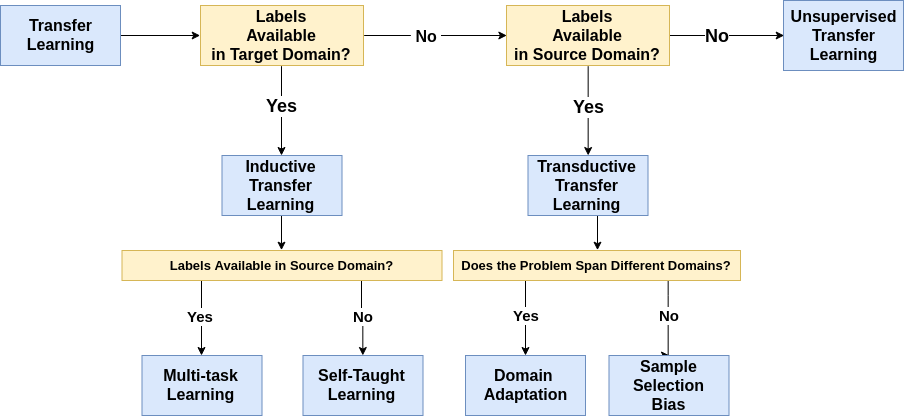
\includegraphics{transfer_learning/transfer-learning-tasks.png}
  \caption{Transfer learning approaches vary  depending on the availability of labeled data for the source and target tasks.}
  \label{fig:transferlearning_models}
\end{figure}

The above approaches vary on what data is available for the learning task - conversely, this also affects what knowledge can be transferred across tasks. 

For example, it is sometimes impossible to apply a source task's data directly to a target task. Instead we can attribute selected instances or features from the source task, which are in turn re-weighted and re-distributed to fit the target task. These methods are referred to as Instance Transfer and Feature-representation Transfer approaches.

In cases where labels are available for either source tasks or target tasks (both inductive and transductive transfer learning), some forms of instance-transfer and feature-representation transfer are possible. Moreover, unsupervised transfer learning techniques are limited to feature-representation transfer \citep{panyang2010}. 

Other examples of transfer learning include broader knowledge transfers such as parameter transfer (or model transfer), where full or parts of parameterized models are transferred from the source task to the target task; or relational-knowledge transfer, where relationships between data points within the source task are transferred to re-distribute data within the target task \citep{cook2013}.   Such transfer is only possible where the target task's labels are available.


\begin{table}[ht]
\centering
\footnotesize
\fontfamily{ppl}\selectfont
\begin{tabular}{llll}
\hline
                                                                           & \begin{tabular}[c]{@{}l@{}}Inductive \\ Transfer Learning\end{tabular} & \begin{tabular}[c]{@{}l@{}}Transductive \\ Transfer Learning\end{tabular} & \begin{tabular}[c]{@{}l@{}}Unsupervised \\ Transfer Learning\end{tabular} \\ \hline
\begin{tabular}[c]{@{}l@{}}Instance \\ Transfer\end{tabular}               & X                                                                      & X                                                                         &                                                                           \\ \hline
\begin{tabular}[c]{@{}l@{}}Feature-representation \\ Transfer\end{tabular} & X                                                                      & X                                                                         & X                                                                         \\ \hline
\begin{tabular}[c]{@{}l@{}}Parameter \\ Transfer\end{tabular}              & X                                                                      &                                                                           &                                                                           \\ \hline
\begin{tabular}[c]{@{}l@{}}Relational-knowledge \\ Transfer\end{tabular}   & X                                                                      &                                                                           &                                                                           \\ \hline
\end{tabular}
\caption{Transfer types by Approach}
\end{table}

\section{Deep Transfer Learning Techniques}\label{sec:transfer-learning-deep-techniques}\index{transfer learning!deep transfer learning techniques}

The above approaches have manifested themselves in two major techniques of transfer learning within deep learning. Multi-layer neural networks are built in such a way that lower-level layers address generic features and higher-level layers address more complex and specific features. The initial layers for a group of related tasks are similar if not identical; this characteristic can be exploited to enable the transfer of knowledge between models \citep{yosinski2014}. 



Off-the shelf models, or pre-trained models, involve training one or more multi-layer networks and adapting parts of the model to another target task. The source models act as a form of pre-training, to learn shallow parts of the problem, while the target learning task is solely limited to the final layer of the model. In fact, one application of pre-trained models can be seen as a feature-selection process \citep{zhu2018}. 

\begin{marginfigure}
  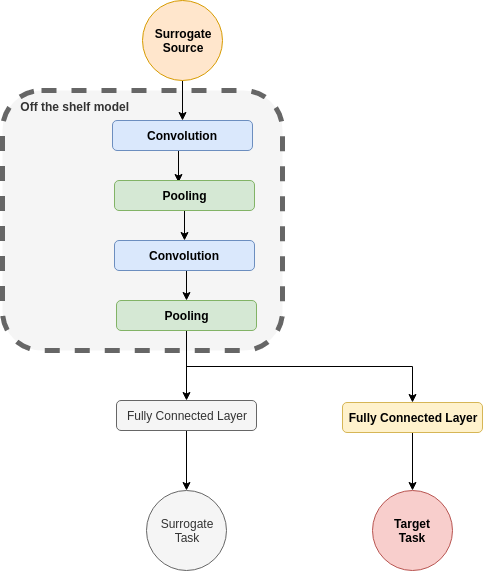
\includegraphics{transfer_learning/transfer-learning-off-the-shelf.png}
  \caption{In off-the-shelf pre-trained models, we replace the final layer of the neural network.}
  \label{fig:transferlearning_pretrained_ots}
\end{marginfigure}

Another approach is to use transfer learning to replace selective parts of the model, rather than just the final layer, this is referred to as model Fine-tuning. 

With Fine-tuning techniques, we pre-train a model using a number of different source tasks, and then re-train the model for the target task; however the target training is done selectively, selecting which layers are to be frozen (and thus inherited from the source tasks) or fine-tuned (to be updated during the backpropagation process). We can define a metric to decide the learning rate for each layer, creating a variable degree of freezing and fine-tuning \citep{madhavan2016}. 

\begin{marginfigure}
  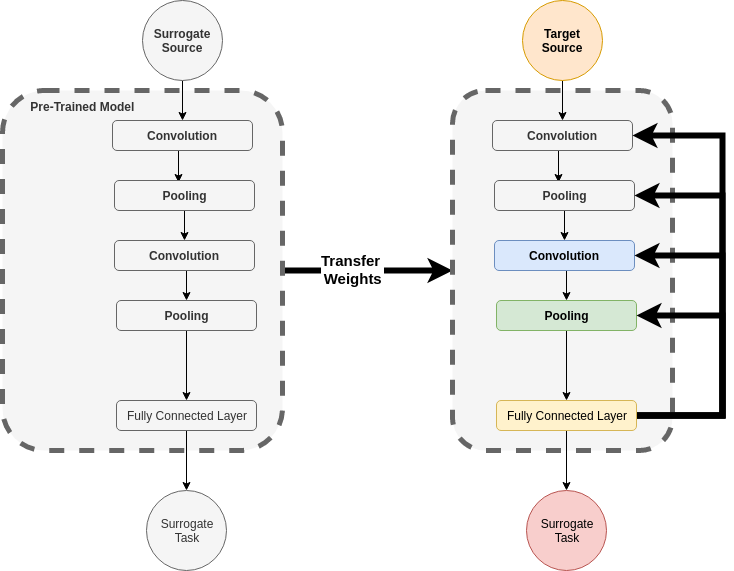
\includegraphics{transfer_learning/transfer-learning-fine-tuning.png}
  \caption{In Pre-trained model fine tuning, we use the source model to initialize the neural network, and fine-tune it using backpropogation.}
  \label{fig:transferlearning_pretrained_finetuning}
 
\end{marginfigure}

The success of transferability is highly dependent on source task's level of specialization, successful transfer learning projects work on generalized source tasks. As a matter of fact, transfer learning across tasks which are too dissimilar as a result of being too specific would result in a negative learning \citep{rosenstein2005}.

\begin{marginfigure}
  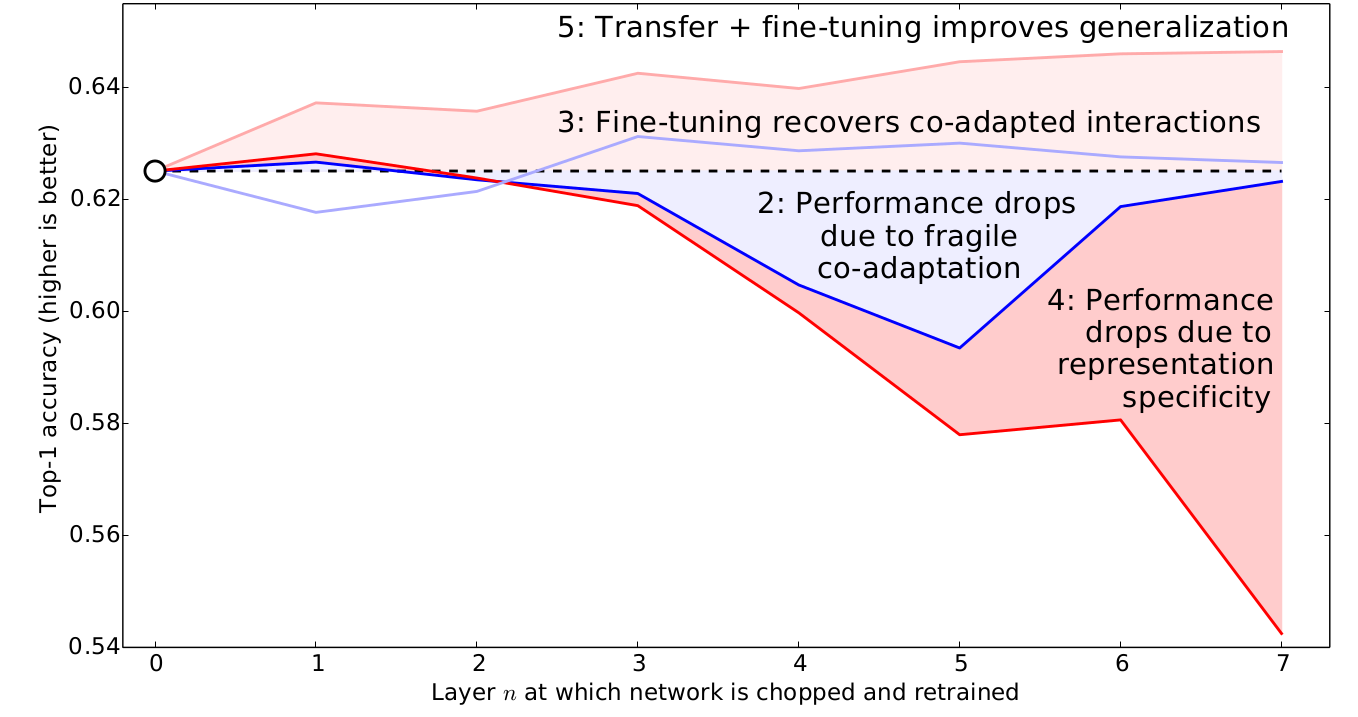
\includegraphics{transfer_learning/transfer_learning_layer_transfer.jpg}
  \caption{The performance gained form fine-tuning a neural network is only relative to the layer generalization and specificity of each distinct layer \citep{yosinski2014}.}
  \label{fig:transferlearning_pretrained_finetuning}
\end{marginfigure}

\section{Applications and Improvements}\label{sec:transfer-learning-applications-improvements}\index{transfer learning!applications and improvements}

Notwithstanding savings on time and computational resources, the above techniques for transfer learning in multi-layer neural networks frequently render better results when compared to training the neural networks from scratch \citep{yosinski2014}. This is especially the case in fields where data collection and annotation is notoriously difficult, such as computer vision and natural language processing. 

The use of pre-trained models machine learning has achieved new state-of-the-art results in several tasks; within the field of computer vision, in object detection \citep{he2017}, semantic segmentation \citep{zhao2016}, human pose estimation \citep{papandreou2017} and action recognition \citep{carreira2017} ; and within the field of natural language processing in text classification, question answering, language inference and conference resolution amongst others \citep{howard2018} \citep{joshi2018}. 

\index{transfer learning|)}
